\section{Numerical Results}
\subsection{2D Rotation}
\label{sec:num-results-2d-rotation}

This test, adapted from \cite{favrie-2014}, considers the evolution of a two-dimensional rotational flow initially confined within a circular region. 
The purpose of the test is to assess the method’s ability to capture strong shear at the interface between rotating and stationary material, as well as to verify the preservation of vorticity constraints inherent to the governing equations.

\begin{figure}[!htp]
   \centering
   \includegraphics[width=0.45\textwidth]{images/2d-rotation.png}
   \caption{2D rotation initial setup.}
   \label{fig:2d-rotation-setup}
\end{figure}

The computational domain is $\left(-L, L\right)^2$, discretized by a uniform Cartesian mesh. 
The initial configuration consists of a circular region of radius $R = 0.05\,\mathrm{m}$ centered at the origin. 
Here, $L$ is chosen as $3R$, as illustrated in Figure~\ref{fig:2d-rotation-setup}, so that the shock does not interact with the boundary.
The velocity field is prescribed as a rigid-body rotation inside the circle and zero elsewhere:
\begin{equation}
  (u,v) =
  \begin{cases}
    (-\omega y,\, \omega x), & \text{if } x^2 + y^2 < R^2, \\[0.4em]
    (0,0), & \text{otherwise},
  \end{cases}
  \label{eq:rotation-init}
\end{equation}
with $\omega = 4\times10^4\,\mathrm{s^{-1}}$. The initial Cauchy stress tensor is spherical,
\[
  \boldsymbol{\sigma} = -p_0 \mathbf{I},
\]
with constant pressure $p_0 = 10^5\,\mathrm{Pa}$. 
The material parameters correspond to aluminum and are given by
\[
  \gamma = 3.4, \quad
  p_\infty = 21.5\,\mathrm{GPa}, \quad
  \mu = 26\,\mathrm{GPa}, \quad
  \rho_0 = 2700\,\mathrm{kg/m^3}.
\]

At the interface $x^2 + y^2 = R^2$, the tangential velocity exhibits a discontinuity, jumping from $2000\,\mathrm{m/s}$ to $0\,\mathrm{m/s}$. 
This strong shear generates both longitudinal and transverse shocks propagating inward and outward from the interface. 
The transverse shocks are of the rarefaction type, where the density decreases behind the front. 
Results are examined at final time $t = 5\,\mu\mathrm{s}$ and are presented in Figure \ref{fig:2d-rotation-density-pressure}.

\begin{figure}
   \centering
   \includegraphics[width=0.45\textwidth]{images/elastic-2d-rotation-NH-density-tfp000005.png}
   \includegraphics[width=0.45\textwidth]{images/elastic-2d-rotation-Aortic-pi4-density-tfp000005.png}
   \caption{Density at $t_f = 5\,\mu\mathrm{s}$. Left: Neo-Hookean model. Right: Aortic model with $\theta = \frac{\pi}{4}$.}
   \label{fig:2d-rotation-density-pressure}
\end{figure}
\MS{Compute vorticity?}

% To assess the preservation of the vorticity constraint, Favrie and Gavrilyuk computed the circulation of the vector $\mathbf{e}_\beta = (a_1,b_1)$ along the closed contour $C$ bounding the domain $D$:
% \begin{equation}
%   \Gamma = \oint_C a_1\,dx + b_1\,dy
%   = \iint_D \left( \frac{\partial b_1}{\partial x} - \frac{\partial a_1}{\partial y} \right) dx\,dy.
%   \label{eq:rotation-circ}
% \end{equation}
% The contour $C$ is taken as the boundary of the square domain of length $L=1\,\mathrm{m}$. 
% The convergence of $\log|\Gamma|$ with grid refinement (using $100\times100$, $200\times200$, $400\times400$, $800\times800$, and $1500\times1500$ meshes) confirmed first-order accuracy of the splitting scheme and demonstrated that the numerical method preserves the vorticity constraint $\nabla \times \mathbf{e}_\beta = 0$ at the discrete level.
